\documentclass[11pt,conference]{IEEEtran}

\usepackage[utf8]{inputenc}
\usepackage[T1]{fontenc}
\usepackage{amsmath}
\usepackage{amssymb}
\usepackage{booktabs}
\usepackage{array}
\usepackage{graphicx}
\usepackage[colorlinks=true, linkcolor=blue, citecolor=blue, urlcolor=blue]{hyperref}
\usepackage{xcolor}
\usepackage{textcomp}
\usepackage{enumitem}
\usepackage{tikz}
\usetikzlibrary{positioning,arrows.meta}

\setlength{\parskip}{3pt plus 1pt minus 1pt}
\setlist{itemsep=2pt, topsep=3pt, parsep=0pt}

\newcommand{\code}[1]{\textit{#1}}

\begin{document}

\title{Predictive Keyboard: N-gram and LLM Blending for Next-Word Prediction}
\author{6738010521 Krittitee Naulkhao, 6738087921 Nutdanai Sikkhakul}
\maketitle

\begin{abstract}
Given a left context and the first letter of the next word, we predict the
word. The pipeline routes by answer type --- symbol (near-deterministic from
the first letter), number (digit-length classification), word
(open-vocabulary, the main task, 88\% of rows) --- and for words blends a
KenLM 5-gram (KN5) with a LoRA-fine-tuned Qwen2.5-3B and zero-shot
Mistral-7B-v0.1, teacher-forced-scored on a shared candidate set. An early
wrong data split was discarded; its findings are reused below only where
still valid (corpus-cleaning and n-gram order/interpolation). Negative
results are reported alongside what worked: stripping punctuation hurts
rather than helps n-gram accuracy, an in-domain+Gigaword interpolated n-gram
still trails the in-domain model alone, and reranking the LLM's own beam
(frozen and trained) never beats the beam's unreranked top1. Final
full-scale, held-out result: \textbf{78.60\% overall / 76.09\% word accuracy
(\textpm0.8pt, 95\% CI)}, submitted as \code{test\_set\_pred.txt}.
\end{abstract}

\section{Data}
\label{sec:data}

\textbf{Official split}: \code{train\_final.src.tok} (3,803,957 lines, 126.65M
tokens, 99,018-word vocab), \code{dev\_set\_final.csv} (94,488 rows),
\code{test\_set\_no\_answer\_final.csv} (94,826 rows). Context/answer length
is long-tailed but thin (p50/p90/p99 = median/90th/99th-percentile token
count): train sentence length p50=33, p90=44, p99=57 tokens; dev context
length p50=24, p90=33, p99=42 --- 99\% of sentences stay under 60 tokens even
though the max reaches 135. N-gram order is therefore never
context-length-bound --- even a 5-gram has plenty of room in a median context.

Train's vocabulary covers dev/test almost completely: baseline dev OOV is
0.13\%, and it stays low under aggressive pruning --- dropping the rarest 50\%
of train's vocab (keeping only words with count $>$23) still costs just 0.47\%
dev OOV, and dropping 70\% still only reaches 1.06\%. The tail is thin and
prunable, not a coverage risk.

\textbf{Answer categories} (regex on the answer token): digits $\rightarrow$
\textbf{number}, \texttt{[a-z']+} $\rightarrow$ \textbf{word}, everything else
(punctuation, and mixed alphanumeric such as a digit+letter token) $\rightarrow$
\textbf{symbol}. Symbol is near-fully deterministic from the given first
letter alone ($\sim$99.6\% majority-vote ceiling; grouping dev's first
letters into 27 buckets (a--z, digit), 24 map to a single answer category
100\% of the time, only \code{1}, \code{e}, \code{u} have rows split across
categories) --- no model needed. Number answers are anonymized to a run of \texttt{1}s
matching the true digit count (\code{2020}$\to$\code{1111}), so number
prediction is really a \textbf{digit-length classification problem}, not text
generation; every number's first letter is literally \code{1}, so this route
is triggered unambiguously. Word is the open-vocabulary main task (83,228 /
94,488 dev rows, 88\%) and is where essentially all modeling effort went.

\textbf{Gigaword} (NYT, 2.37GB compressed,
$\sim$1.4B tokens after masking to train's vocab) was tried as extra general
training data. It does not fit the task: after masking, its own vocab
(93,279 words) is \emph{smaller} than train's (99,018) despite roughly 8x the
lines, and a 4-gram trained on it alone underperforms training on
\code{train\_final.src.tok} alone by 9.9pt overall / 10.3pp alphanumeric
(\S\ref{sec:ngram}) --- off-domain text does not cover dev/test's specific
distribution even after vocab-masking and retokenizing. Gigaword was
ultimately kept only as an auxiliary corpus for the number category, where
its scale outweighs the domain mismatch because the sub-task (digit-length
only, \S\ref{sec:kn5number}) is narrow enough for out-of-domain text to still
help.

\textbf{Cleaning hypothesis} We have assumption going in that stripping
punctuation before training would reduce n-gram sparsity (fewer distinct
context "words" ending in \texttt{,}/\texttt{-}) and so improve word accuracy.
Tested directly, one variable at a time, with punctuation stripped from both
the training corpus and the dev context (so this is not a
train/eval-format mismatch): a corpus cleaned to alphanumeric-only scores 45.19\%
vs.\ 51.71\% raw (\textbf{-6.5pp}). Since both sides were cleaned
consistently, 
it is evidence that punctuation tokens in the context carry real predictive
structure (e.g.\ marking clause boundaries and syntactic position) that the
n-gram uses, not just noise diluting the counts. Resulting in us using raw text for every
n-gram from this point on.

\section{Model}

\subsection{N-gram}
\label{sec:ngram}

Two n-gram models with fallback to lower order recur throughout this section, on both the discarded split
and the official data: \textbf{Model A} is trained on the task's own,
in-domain train corpus (
\code{train\_final.src.tok} on the official data); \textbf{Model B} is
trained on Gigaword instead, vocab-masked to Model A's vocabulary so the two
are directly comparable. Model A is the in-domain model and Model B is the
out-of-domain one.

\textbf{Order and fallback rate.} Order 4--5 was chosen from a fallback-rate
check, not context length. At order 4, pruned \code{(context, word)} tables
already hit their fallback for 98.0\% of
contexts (54.8\% at order 2, 94.1\% at order 3). Separately, on the discarded
split, pushing Model A alone from order 4 through order 7 measured this
diminishing-returns curve directly:

\begin{table}[h]
\centering
\caption{N-gram order vs.\ accuracy (Model A, discarded split)}
\label{tab:order}
\begin{tabular}{lrr}
\toprule
order & eval accuracy & test accuracy \\
\midrule
4 & 57.00\% & 56.73\% \\
5 & 57.61\% & 57.47\% \\
6 & 57.74\% & 57.81\% \\
7 & 57.81\% & 57.86\% \\
\bottomrule
\end{tabular}
\end{table}

Order 6 gains +0.13pp over 5, order 7 gains another +0.07pp over 6 ---
monotonic but shrinking, confirming order 5 is near the plateau; not worth
chasing order 8/9.

\textbf{Model A + Model B interpolation.} Linear
interpolation in probability space, $P = \lambda A +
(1-\lambda) B$, was grid-searched for $\lambda$ against
perplexity on eval dataset, then applied as-is to test and to the accuracy task. Best
$\lambda=0.71$ cut perplexity by $\sim$20\% over Model A alone (92.3
$\rightarrow$ 74.0) and carried straight over to accuracy without separate
tuning: alphanumeric accuracy rose from 57.61\%/57.47\% (Model A solo) to
\textbf{60.16\%/60.02\%} (eval/test) --- a further +2.5--2.6pp gain, the
biggest lever in the n-gram stage.

\textbf{Engine: Python to C++.} The first trainer was a pure-Python count
table, which OOMs on gigaword-sized corpora --- it does not scale past the
train-only corpus. Replaced with
\textbf{KenLM} (C++, exact external-memory counting, modified Kneser--Ney
smoothing) --- this became the production n-gram engine (\code{KN5}, trained
on the full 130M-token official train corpus) for every experiment after
this point, including the LLM blends below.

\textbf{KN5 as the blend's scorer.} Up to this point the LLM blend's n-gram
term (\S\ref{sec:llm}) was an unsmoothed relative-frequency count scorer with
plain order-4-to-1 backoff. It was swapped for \textbf{KN5} --- modified-Kneser-Ney smoothing on the full
130M-token train corpus --- so the blend's n-gram signal gets properly
calibrated (smoothed, backoff-discounted) log-probabilities instead of raw
counts, at no extra inference cost.
Compared under the identical pooled-CV blend harness, swapping only the
n-gram scorer: 71.52\%$\to$\textbf{71.74\%} word, 74.47\%$\to$\textbf{74.66\%}
overall (+0.22pp / +0.19pp) --- real but small, since the blend's ceiling is
set mostly by the candidate set (LM beam top5 $\cup$ n-gram top1) rather than
by how well-calibrated either side's probabilities are. Kept as the default
scorer regardless, since it is strictly better for free.

\textbf{Dedicated number KN5.}
\label{sec:kn5number}
Numbers have few in-domain training examples making the n-gram comparatively weak so we built a second KN5 trained
\emph{only} on number-containing lines: gigaword paragraphs with $\geq$1 digit
token (anonymized all integer to \code{1}) plus
train's own number-containing lines, 11.56M lines / 606M tokens combined.
This is the one place gigaword's raw scale helps rather than hurts, since the
sub-task is narrow enough that off-domain text about numbers still transfers.
Result: 71.97\% $\rightarrow$ \textbf{74.59\%} number accuracy (+2.6pp),
beating a same-corpus-subset baseline .

\subsection{Large Language Model}
\label{sec:llm}

\textbf{Choosing a base model.} The shortlist itself was drawn from public
leaderboard scores (HellaSwag, cross-validated against ARC and MMLU) as a
cheap proxy for general capability, initially favoring Mistral-7B-v0.1. Since
none of those benchmarks match this task's format, every candidate was
then benchmarked zero-shot directly on the task itself (2,000-row sample,
greedy decoding, letter-masked), which overturned the leaderboard ranking ---
Qwen2.5-3B was chosen as base model because it is much smaller than
Mistral-7B-v0.1 yet performs slightly ahead on the real task.

\begin{table}[h]
\centering
\caption{Zero-shot model shortlist (2000-row sample, greedy, letter-masked)}
\label{tab:shortlist}
\begin{tabular}{lrr}
\toprule
model & word acc.\ & overall \\
\midrule
\textbf{Qwen2.5-3B} (kept) & \textbf{70.26\%} & \textbf{71.55\%} \\
Mistral-7B-v0.1 & 69.92\% & 71.25\% \\
granite-3.1-2b-base & 68.10\% & 69.65\% \\
Qwen2.5-1.5B & 67.99\% & 69.55\% \\
gemma-2-2b & 67.99\% & 69.55\% \\
Qwen3.5-4B-Base & 66.46\% & 68.45\% \\
Falcon3-3B-Base & 61.92\% & 64.20\% \\
SmolLM2-1.7B & 61.07\% & 63.45\% \\
phi-2 & 59.08\% & 62.15\% \\
\bottomrule
\end{tabular}
\end{table}

The spread is 11pp top-to-bottom among models all under 7B parameters:
Falcon3-3B-Base, SmolLM2-1.7B and phi-2 in particular trail the winner by
8--11pp despite being the same size class or larger than some models that did
well, so parameter count alone did not predict this task's zero-shot
accuracy --- pretraining data/recipe mattered more. A later check of Qwen3.5
confirmed newer/bigger was not automatically better here either:
Qwen3.5-4B-Base scored 66.46\% word and Qwen3.5-2B-Base 61.18\%, both below
Qwen2.5-3B's 70.26\%, and 2.5--4x slower per row in this environment. Qwen2.5-3B
was kept as the base model throughout.


\textbf{From-scratch GPT-2.} As a fourth, non-pretrained comparison point, a
GPT-2-medium-widened model (497M params, word-level vocab built directly from
train, no subword/BPE, never pretrained) was trained from random
initialization on the full corpus to a
flat loss plateau. It reached \textbf{68.09\% alphanumeric} (71.45\% overall,
test split) --- close to the zero-shot pretrained 3B models, but plateaued there. 
Conclusion: This is roughly the ceiling for a from-scratch model at this corpus size.

\textbf{Fine-tuning Qwen2.5-3B, matched protocol.} Qwen2.5-3B (LoRA,
r=16/$\alpha$=32, on q/k/v/o\_proj, plain packed-sequence causal-LM
objective) was fine-tuned on the full train corpus. Under matched greedy
decoding, the zero-shot base model scores 70.20\% word
(Table~\ref{tab:shortlist}); the fine-tuned checkpoint reaches
\textbf{73.15\%} (+2.95pp) --- fine-tuning measurably helps beyond the
pretrained zero-shot baseline.

\textbf{Error analysis on the fine-tuned model.} On a beam-k5 evaluation of
this checkpoint, of the 2,482/8,198 word rows still wrong at top1: 100\%
start with the correct letter (the mask is doing
its job, every miss is a within-letter ranking error); 47\% are recovered by
top5 (already in the beam, just ranked below \#1); the dominant failure mode
is genuine function-word ambiguity unknowable from left context alone
(a$\leftrightarrow$an, that$\to$to, and$\to$at, their$\to$the); a smaller
share is unknowable factual choice (sunday$\to$saturday) or a register
mismatch (informal \code{u}$\to$\code{us}). Accuracy by first letter tracks
branching factor, not the letter itself --- worst are high-branching
consonant starts (r, u, g, s, c: 58--61\% top1), best are rare or
low-branching starts (x, y, o, z, t: 79--100\% top1).

\textbf{Rerankers --- tried, both hurt.} Two rerankers over the fine-tuned
model's top5 beam were tried: a frozen \code{MiniLM} cosine-similarity
reranker (58.31\% top1) and a \code{MiniLM} cross-encoder trained
specifically for this reranking task (62.34\% top1) --- both below the
beam's own unreranked top1. A reranker only ever sees the same left-context
the causal LM already conditioned on, so at best it is a smaller, worse copy
of the ranking the LLM's own beam search already computes for free.

\textbf{Direct (teacher-forced) candidate scoring.} Every candidate in a widened
union set (LM top5 $\cup$ n-gram top10 for that letter) was scored with one
batched teacher-forced forward pass, summing full-word log-probability. This
removes beam-search pruning distortion on multi-subword words and lets scores
be compared directly across candidates the beam itself never fully explored:
71.74\% $\to$ \textbf{72.62\%} word (+0.88pp), 74.66\% $\to$ \textbf{75.42\%}
overall (+0.76pp) --- the largest gain among the candidate-scoring changes.

\textbf{2-way blend.} Combining the fine-tuned Qwen2.5-3B with KN5,
teacher-forced scoring on both sides:
\begin{equation}
\text{score}(w) = \lambda \cdot \text{qwen}_{tf}(w) + (1-\lambda) \cdot \text{kn5}(w)
\label{eq:blend2}
\end{equation}
reached \textbf{72.62\%} word / \textbf{75.42\%} overall (pooled 5-fold CV,
every row held out exactly once) --- beating fine-tuned Qwen alone by
+2.9pp word; the pooled-CV number for the pre-KN5 scorer was 71.52\%.

\textbf{3-way blend, adding Mistral.} Rather than fine-tuning a second model,
\textbf{Mistral-7B-v0.1 base, zero-shot}, was teacher-forced-scored on the
\emph{exact same} candidate set already fixed for Qwen (no new beam search or
candidate generation for Mistral at all):
\begin{equation}
\begin{split}
\text{score}(w) = &\ \lambda_q \cdot \text{qwen}_{tf}(w) + \lambda_m \cdot \text{mistral}_{tf}(w) \\
&+ (1-\lambda_q-\lambda_m) \cdot \text{kn5}(w)
\end{split}
\label{eq:blend3}
\end{equation}
Mistral was chosen for architectural diversity, not solo accuracy: two other
different architectures were checked first, state-space \code{mamba-2.8b}
(65.55\% word zero-shot) and pure-RNN \code{RWKV-4-3b} (60.66\%), but both
trailed Qwen by 4.7--9.6pp, too far behind to expect a net blend gain;
Mistral was chosen instead, only -0.34pp behind Qwen solo. The 3-way blend
gave the largest gain among the blending experiments: 74.64\% $\rightarrow$
\textbf{75.09\%} word, 77.18\% $\rightarrow$ \textbf{77.68\%} overall (after
a later continued fine-tune and wider beam, below), a +2.0pp word jump from
adding Mistral alone: its errors are decorrelated enough from Qwen's that
the blend weights it more than raw solo accuracy would predict.

\textbf{Wider beam for candidate generation.} Candidate generation was
widened from a k=5 to a k=10 beam on the fine-tuned checkpoint above ---
error analysis had found 9.5\% of word rows hit a hard candidate-set ceiling
at k=5, so this targets that directly (candidate-set coverage: top5 84.02\%
$\to$ \textbf{87.57\%}, top10 88.13\%, same sample). Re-running the full
3-way blend on the widened candidate set: 74.64\% $\to$ \textbf{75.09\%}
word, 77.29\% $\to$ \textbf{77.68\%} overall.

\subsection{Final full-scale run}
\label{sec:final}

\begin{center}
\resizebox{\columnwidth}{!}{%
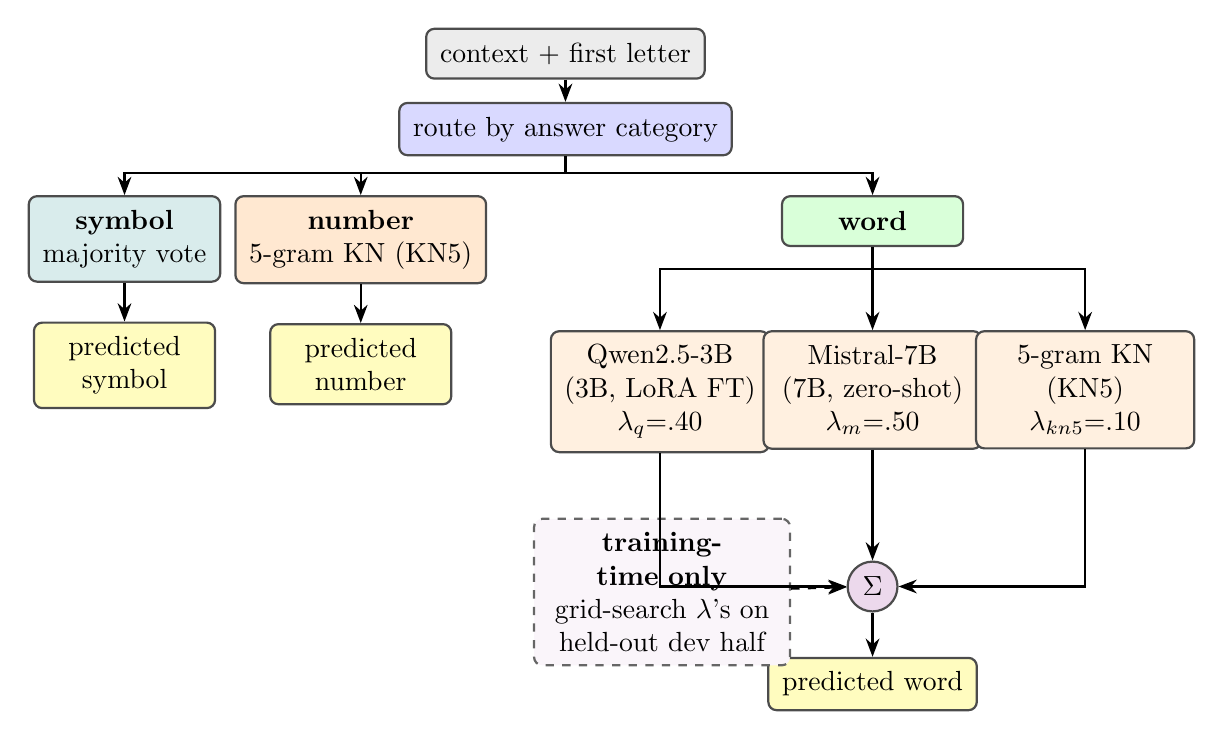
\begin{tikzpicture}[
  every node/.style={font=\normalsize},
  box/.style={draw=black!70, thick, rounded corners=3pt, align=center,
              inner sep=5pt, minimum height=18pt, minimum width=2.3cm,
              fill=blue!6},
  small/.style={box, text width=2.7cm, minimum width=2.7cm, inner xsep=1pt, fill=orange!12},
  sum/.style={draw=black!70, thick, circle, fill=violet!15, inner sep=1pt,
              minimum size=18pt, font=\normalsize},
  train/.style={draw=black!60, thick, dashed, rounded corners=3pt, align=center,
                inner sep=5pt, minimum height=18pt, text width=2.9cm, fill=violet!4},
  >=Stealth, node distance=8pt and 7pt,
  every path/.style={thick},
]
\node[box, fill=gray!15] (in) {context + first letter};
\node[box, below=of in, fill=blue!15] (route) {route by answer category};
\node[box, below=14pt of route, xshift=-5.6cm, fill=teal!15] (sym) {\textbf{symbol}\\majority vote};
\node[box, below=14pt of route, xshift=-2.6cm, fill=orange!18] (num) {\textbf{number}\\5-gram KN (KN5)};
\node[box, below=14pt of route, xshift=3.9cm, fill=green!15] (word) {\textbf{word}};
\node[box, below=14pt of sym, fill=yellow!25] (outsym) {predicted\\symbol};
\node[box, below=14pt of num, fill=yellow!25] (outnum) {predicted\\number};
\node[small, below=30pt of word, xshift=-2.7cm] (qwen) {Qwen2.5-3B\\(3B, LoRA FT)\\$\lambda_q$=.40};
\node[small, below=30pt of word] (mistral) {Mistral-7B\\(7B, zero-shot)\\$\lambda_m$=.50};
\node[small, below=30pt of word, xshift=2.7cm] (kn5w) {5-gram KN\\(KN5)\\$\lambda_{kn5}$=.10};
\node[sum, below=40pt of mistral] (sigma) {$\Sigma$};
\node[box, below=16pt of sigma, fill=yellow!25] (out) {predicted word};
\node[train, left=20pt of sigma, yshift=-2pt] (tune) {\textbf{training-time only}\\grid-search $\lambda$'s on held-out dev half};
\draw[->] (in) -- (route);
\draw[->] (route.south) -- ++(0,-6pt) -| (sym.north);
\draw[->] (route.south) -- ++(0,-6pt) -| (num.north);
\draw[->] (route.south) -- ++(0,-6pt) -| (word.north);
\draw[->] (sym) -- (outsym);
\draw[->] (num) -- (outnum);
\draw[->] (word.south) -- ++(0,-8pt) -| (qwen.north);
\draw[->] (word.south) -- (mistral.north);
\draw[->] (word.south) -- ++(0,-8pt) -| (kn5w.north);
\draw[->] (qwen.south) |- (sigma.west);
\draw[->] (mistral.south) -- (sigma.north);
\draw[->] (kn5w.south) |- (sigma.east);
\draw[->] (sigma) -- (out);
\draw[->, dashed] (tune) -- (sigma);
\end{tikzpicture}%
}
\end{center}

The comparison-track numbers above are all measured on a fixed 10\% dev
sample (9,448 rows) for fast iteration. The actual submission pipeline was
run at full scale. Due to compute constraints, inference was split across
multiple machines running in parallel and merged back by absolute row index.
\begin{itemize}
\item Dev was stratified-subsampled 94,488 $\to$ 20,000 rows (seed 123,
proportional per answer category) to bound total inference time; test was
run in full (94,826 rows).
\item Qwen and Mistral scoring both ran split across the available
machines, merged back by absolute row index before blending.
\end{itemize}

$\lambda$ was tuned on one stratified half of the 20,000-row dev subsample
(n=10,001) and accuracy reported on the other, untouched half (n=9,999) ---
the same held-out discipline as the pooled-CV protocol above, a single 50/50
split rather than 5-fold since 20k rows already gives a tight interval
without needing the extra folds.

\begin{table*}[!t]
\centering
\large
\caption{Final full-scale result (submitted)}
\label{tab:final}
\begin{tabular}{lrr}
\toprule
category & accuracy & 95\% CI (Wilson) \\
\midrule
word & 76.09\% (6602/8676) & [75.19\%, 76.98\%] \\
symbol & 99.10\% (1099/1109) & [98.35\%, 99.51\%] \\
number & 73.83\% (158/214) & [67.56\%, 79.26\%] \\
\midrule
\textbf{overall} & \textbf{78.60\% (7859/9999)} & \textbf{[77.78\%, 79.39\%]} \\
\bottomrule
\end{tabular}
\end{table*}

Final blend weights: $\lambda_{qwen}=0.40$, $\lambda_{mistral}=0.50$,
$\lambda_{kn5}=0.10$. This run produced the submitted \code{test\_set\_pred.txt}
(94,826 predictions, full test set).

CIs are Wilson score intervals at $z=1.96$ (95\% confidence).

\section{Conclusion}

Most of the starting assumptions, tested directly, came back wrong: corpus
cleaning hurts the n-gram rather than helping it (\S\ref{sec:data}); reranking the LLM's
beam (\S\ref{sec:llm}) underperformed the beam's own ranking; per-letter
(sub-category) $\lambda$ tuning did no better than one global $\lambda$ per
model. In each case the "extra" signal turned out to be redundant with what
the LM/n-gram log-probs already encoded, not independent of it --- added
model complexity only pays off when the new feature carries information the
existing signal doesn't already have.

Blending two models from the \emph{same} trained lineage (e.g.\ two
checkpoints of the same fine-tuned architecture) tends to collapse one
weight toward zero --- no new information to add. The gain came specifically
from blending a fine-tuned model with an architecturally different,
independently-pretrained zero-shot model (Mistral, weighted \emph{more} than
Qwen in the final blend despite lower solo accuracy).

\textbf{Challenges.} Compute was the main constraint --- roughly 50 GPU-hours
on Kaggle T4$\times$2 plus 10+ hours local. The final inference run split
work across both Kaggle and local machines in parallel, merged back
afterward; the n-gram trainer was moved from pure Python to the C++ KenLM
implementation to handle gigaword-scale data.

\textbf{What we'd do better.} The zero-shot spread in
Table~\ref{tab:shortlist} (11pp between Qwen2.5-3B and phi-2, all under 7B)
tracks pretraining scale/recipe more than any pipeline choice tested here,
so a larger base model is the most direct untested lever toward 80\% overall.

\begin{table*}[p]
\centering
\large
\caption{All methods tried, roughly in the order they were tried}
\label{tab:results}
\begin{tabular}{lrr}
\toprule
method & word / metric & overall \\
\midrule
n-gram, order-5, cleaned corpus (hyp.\ test) & 45.19\% & --- \\
n-gram, order-5, raw corpus & 57.61\% alphanumeric & --- \\
n-gram, Model A+B interpolated ($\lambda$=0.71) & 60.16\% alphanumeric & --- \\
n-gram, order-4, official data (Model A) & 55.51\% & 60.12\% \\
n-gram, order-4, gigaword only (Model B, official) & 45.17\% & 50.23\% \\
GPT-2 (497M), trained from scratch & 68.09\% alphanumeric & 71.45\% \\
Qwen2.5-0.5B, LoRA fine-tuned, undertrained & 39.83\% alphanumeric & --- \\
small pretrained LLM shortlist, zero-shot & 59--70\% (Table~\ref{tab:shortlist}) & 62--72\% \\
Qwen2.5-3B, zero-shot (matched beam k=5) & 66.52\% & --- \\
Qwen2.5-3B, fine-tuned (LoRA r=16/$\alpha$=32) & 73.15\% & --- \\
2-way blend: Qwen (teacher-forced) + KN5 & 72.62\% & 75.42\% \\
3-way blend: + Mistral zero-shot & 74.64\% & 77.18\% \\
3-way blend: + continued fine-tune, k=10 beam & \textbf{75.09\%} & \textbf{77.68\%} \\
number: general n-gram $\to$ dedicated KN5 & 71.97$\to$74.59\% & --- \\
\textbf{final full-scale run (submitted)} & \textbf{76.09\%} & \textbf{78.60\%} \\
\bottomrule
\end{tabular}
\end{table*}

\end{document}